Suppose that the LIDAR returns a value of $(r, \theta)$ when scanning an object. With reference to Figure 42.5, please express the location of the object with respect to the LIDAR frame L.

\begin{center}
    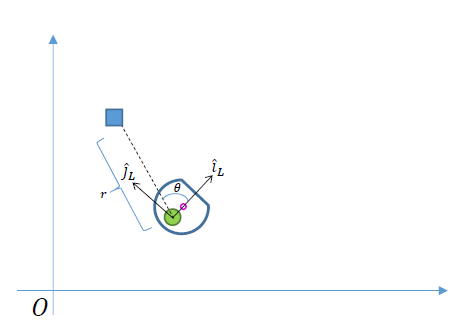
\includegraphics[width=0.75\textwidth]{img/42-5.png}
    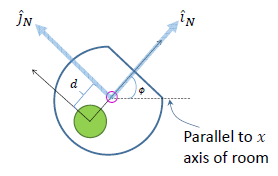
\includegraphics[width=0.4\textwidth]{img/42-6.png}
\end{center}

\begin{solution}
\begin{align*}
    r_L &= r\cos\theta \boldsymbol{\hat{i}}_L + r\sin\theta \boldsymbol{\hat{j}}_L \\
    r_L &= \begin{bmatrix}
        r\cos\theta \\
        r\sin\theta
    \end{bmatrix}
\end{align*}
\end{solution}